\section{Static Pattern Classification on Real World Data}

Dataset 2A consists of image histogram data pertaining to five class labels in which each image is represented by a 24 dimensional feature vector. The training accuracies were found to increase with increasing number of clusters in both cases. The best model was found to require much lower cluster numbers of gaussians in the case of full covariance matrix models compared to diagonal covariance matrix models. 

 The optimal model for diagonal covariance matrix model being [5,5,5,5,5], The test accuracy was 50.87$\%$. The optimal model for full covariance matrix model being [4,4,4,4,4] and the test accuracy was 57.23$\%$.


% -----------------------------------------------------------
{\rowcolors{3}{green!40!yellow!10}{green!0!yellow!30}
\begin{table}[!h]
\centering
\begin{tabular}{ |c|c|c|  }
\hline
\rowcolor{lightgray} Model & Training Accuracy & Val Accuracy \\
\hline
[1,1,1,1,1] & 52.41$\%$  & 45.90$\%$ \\   
 \hline
[2,2,2,2,2] & 56.98$\%$  & 40.98$\%$ \\ 
\hline
[3,3,3,3,3] & 60.30$\%$  & 46.99$\%$ \\
\hline
[4,4,4,4,4] & 64.20$\%$  & 49.18$\%$ \\
\hline
[5,5,5,5,5] & 66.55$\%$  & 53.55$\%$ \\
\hline
[8,8,8,8,8] & 73.78$\%$  & 51.36$\%$ \\
\hline
[11,11,11,11,11] & 77.72$\%$  & 49.18$\%$ \\
\hline
\end{tabular}
\caption{Performance of models for Diagonal Covariance matrix}.
\label{table:7}
\end{table}
}
\newpage
% -----------------------------------------------------------
{\rowcolors{3}{green!40!yellow!10}{green!0!yellow!30}
\begin{table}[!h]
\centering
\begin{tabular}{ |c|c|c|  }
\hline
\rowcolor{lightgray} Model & Training Accuracy & Val Accuracy \\
\hline
[1,1,1,1,1] & 68.26$\%$  & 56.28$\%$ \\   
 \hline
[2,2,2,2,2] & 76.21$\%$  & 57.92$\%$ \\ 
\hline
[3,3,3,3,3] & 83.44$\%$  & 58.54$\%$ \\
\hline
[4,4,4,4,4] & 87.26$\%$  & 60.0$\%$ \\
\hline
[5,5,5,5,5] & 91.15$\%$  & 55.71$\%$ \\
\hline
[8,8,8,8,8] & 96.27$\%$  & 51.43$\%$ \\
\hline
[10,10,10,10,10] & 98.56$\%$  & 42.86$\%$ \\
\hline
\end{tabular}
\caption{Performance of models for Full Covariance matrix}.
\label{table:8}
\end{table}
}


\begin{figure}[!t]
    \centering
    \begin{subfigure}[t]{0.5\textwidth}
        \centering
        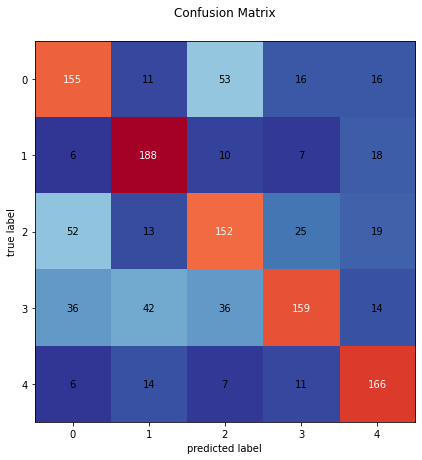
\includegraphics[height=2.5in]{Dataset_2a/train1_diag.png}
        \caption{Train Data}
    \end{subfigure}%
    ~ 
    \begin{subfigure}[t]{0.5\textwidth}
        \centering
        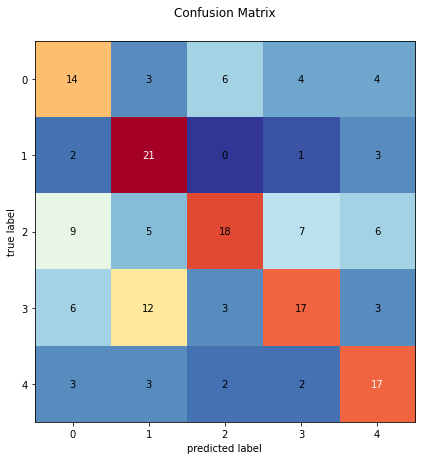
\includegraphics[height=2.5in]{Dataset_2a/test1_diag.png} 
        \caption{Validation Data}
    \end{subfigure}%
    ~
    \caption{Confusion Matrix for diagonal covariance}
    \label{fig:28}
\end{figure}

\newpage
\begin{figure}[!h]
    \centering
    \begin{subfigure}[t]{0.5\textwidth}
        \centering
        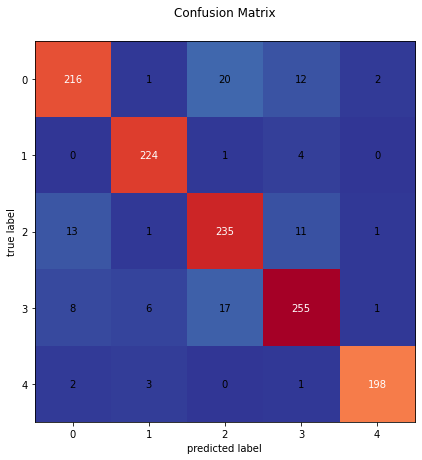
\includegraphics[height=2.5in]{Dataset_2a/train1_full.png} 
        \caption{Train Data}
    \end{subfigure}%
    ~ 
    \begin{subfigure}[t]{0.5\textwidth}
        \centering
        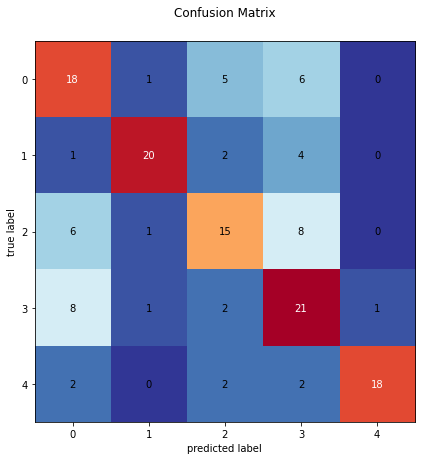
\includegraphics[height=2.5in]{Dataset_2a/test1_full.png}
        \caption{Validation Data}
    \end{subfigure}%
    ~
    \caption{Confusion Matrix for full covariance}
    \label{fig:29}
\end{figure}